\chapter{Les robots parall\`eles \`a c\^ables} \label{chap0}

Il s'agit dans ce chapitre d'introduire les problématiques et méthodologies qui 
nous guideront dans notre étude de l'utilisation de l'asservissement visuel pour 
une architecture de robot très particulière, les robots parall\`eles \`a 
c\^ables. Deux objectifs animent ce travail : il s'agit dans un premier temps 
de perfectionner les fonctionnalités de saisie et manipulation d'objets de ces 
robots, et d'en améliorer les propriétés dans un second temps.

Pour cela, nous  évoquons dans une première section les avantages et 
inconvénients des structures parallèles comparativement aux structures en série. 
Les spécificités des manipulateurs à c\^ables sont introduites dans une deuxième 
section, suivie d'un rappel de leurs modèles géométriques et cinématiques. 
Nous présentons ensuite dans une troisième section la classe des manipulateurs 
de type N-1, \`a laquelle appartient le prototype sur lequel nous avons 
effectu\'e nos expérimentations et validations , et dont nous donnerons 
les principales propri\'et\'es.

%Dans une quatrième section, à la suite d'un rappel des modèles 
%d'asser\-vissement visuel, nous justifierons les choix de configuration 
%d'asservissement que nous avons opérés, et indiquerons de quelles manières 
%notre approche se démarque des travaux existants dans ce domaine précis. En 
%particulier, les robots à câbles peuvent fonctionner selon différents modes ; 
%nous montrerons comment nous avons utilisé cette spécificité pour en optimiser 
%la commande. La cinquième et dernière section présentera les problématiques de 
%l'étude de la manipulation et les choix méthodologiques qui en ont permis la 
%résolution.

\section{Manipulateurs série et parallèles} \label{chap0-0}

C'est incontestablement l'industrie qui aura été le principal vecteur de 
développe\-ment de la robotique ces deux derniers siècles. L'introduction des 
robots dans les usines s'inscrit dans une démarche d'augmentation de la 
productivité et d'amélio\-ration des performances. Cela aura permis dès lors de 
soulager le travailleur humain dans des situations de travail pénible et/ou 
répétitif, et d'augmenter ses compétences en permettant par exemple une 
précision qu'il ne saurait fournir seul, ou la possibilité de déplacer des 
charges élevées. Si la grande diversité que recouvre aujourd'hui le terme de 
{\it robot} rend extrêmement difficile l'élaboration d'une définition générique, 
nous pouvons cependant en dériver des sous-catégories plus faciles à 
appréhender. Parmi celles-ci, nous distinguons en particulier la classe des 
manipulateurs dont l'objectif sera le déplacement et positionnement d'objets 
dans l'espace.

\subsection{Définitions} \label{chap0-0-0}

Un manipulateur sera constitué de manière générale d'une base et d'un organe 
terminal, reliés par une ou plusieurs chaînes cinématiques plus ou moins 
élaborées.

Une chaîne cinématique est caractérisée par une succession de solides reliés 
par des articulations simples ou complexes. Les articulations simples peuvent 
être de nature {\it prismatique} (Fig.\ref{intro:fig0view0}) -- permettant la 
translation d'un solide par rapport à l'autre -- ou {\it rotoïdes} 
(Fig.\ref{intro:fig0view1}) -- effectuant un mouvement de rotation autour d'un 
axe donné. Des articulations complexes sont obtenues à partir de la combinaison 
de mouvements prismatiques et/ou rotoïdes : une articulation cylindrique 
(Fig.\ref{intro:fig0view2}) permet par exemple la combinaison d'un mouvement de 
translation selon un axe donné et d'un mouvement de rotation autour de ce même 
axe ; autre exemple, une articulation sphérique (Fig.\ref{intro:fig0view3}) 
combinera quant à elle trois rotations.

\begin{figure}[!ht]
  \centering
      \subfloat[Articulation simple de type prismatique]{\label{intro:fig0view0}
    
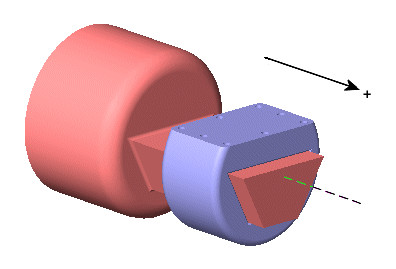
\includegraphics[width=.24\linewidth]{./chapter0/figures/prismaticJoint.jpg}} 
\hfill
    \subfloat[Articulation simple de type rotoïde]{\label{intro:fig0view1}
    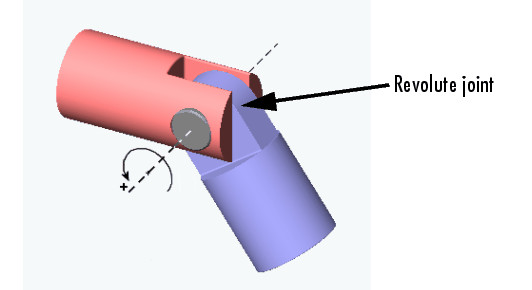
\includegraphics[width=.24\linewidth]{./chapter0/figures/revoluteJoint.jpg}} 
\hfill
  \subfloat[Articulation composée de type cylindrique]{\label{intro:fig0view2}
    
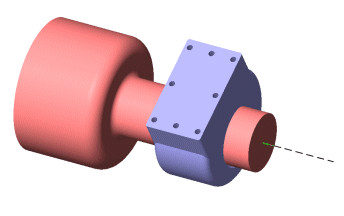
\includegraphics[width=.24\linewidth]{./chapter0/figures/cylindricalJoint.jpg}} 
\hfill
  \subfloat[Articulation composée de type sphérique]{\label{intro:fig0view3}
    
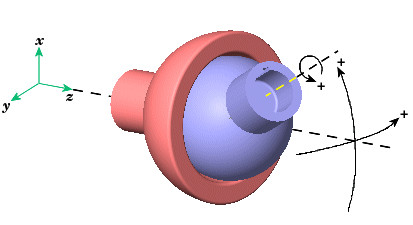
\includegraphics[width=.24\linewidth]{./chapter0/figures/sphericalJoint.jpg}}
    \caption{\footnotesize{Différents exemples d'articulations.}}
\label{intro:fig0}
\end{figure}

On appelle {\it coordonnées articulaires} l'ensemble des valeurs prises par les 
paramètres permettant de décrire l'état des articulations à un instant donné. 
Les coordonnées articulaires sont exprimées dans un espace articulaire propre à 
chaque articulation. Les paramètres nécessaires à l'expression des coordonnées 
articulaires sont généralement au nombre de 3 pour un point (ses coordonnées 
dans l'espace cartésien) et de 6 pour un solide (position cartésienne complétée 
par trois angles de rotation). Le nombre de paramètres non fixés par la 
géométrie du robot et nécessaires à la description exhaustive des coordonnées 
d'une articulation est appelé {\it degré de liberté}. Lorsque les articulations 
ne sont pas laissées libres, leur valeur dans l'{\it espace articulaire} sera 
contr\^olée par des {\it actionneurs} : on distinguera donc les {\it 
articulations actionnées} des {\it articulations passives}.

De la même manière, on parlera des {\it coordonnées opérationnelles} pour 
définir la pose de l'organe terminal, exprimées par rapport à un référentiel de 
référence. A nouveau, nous pouvons définir les degrés de liberté de l'organe 
terminal comme le nombre de paramètres contr\^olés pour le déplacer dans 
l'espace. Cette notion est à distinguer de la mobilité de l'organe terminal, 
qui 
correspond aux possibilités de déplacement de l'organe terminal, contrôlées ou 
laissées libres. Si l'on décide par exemple de contr\^oler les mouvements en 
translation, de bloquer deux rotations mais d'en laisser libre une, la mobilité 
sera de 4, mais le nombre de degrés de libertés ne sera que de 3.

Enfin, on peut définir pour chaque segment son {\it degré de connexion} comme 
étant le nombre de solides auxquels il est relié par une articulation libre ou 
actionnée. Lorsque l'ensemble des segments ont un degré de connexion égal à 2 à 
l'exception de la base et de l'organe terminal qui ont de degré de connexion 
égal à 1, on parle de {\it cha\^ine cinématique ouverte} 
(Fig.\ref{intro:fig1view0}). Lorsque l'un des segments au moins (différent de 
la 
base) possède un degré de connexion supérieur ou égal à 3, nous avons une {\it 
cha\^ine cinématique fermée} (Fig.\ref{intro:fig1view1}) 
\cite{journals/gosselin1989}. Les cha\^ines cinématiques complexes sont 
constituées de plusieurs cha\^ines fermées et/ou ouvertes.

\begin{figure}[!ht]
  \centering
      \subfloat[Schéma d'une cha\^ine cinématique 
ouverte]{\label{intro:fig1view0}
    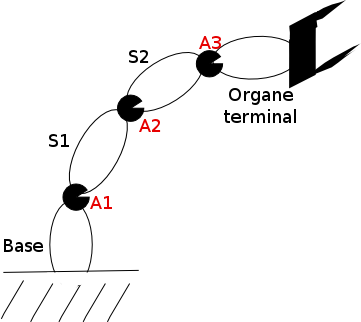
\includegraphics[width=.48\linewidth]{./chapter0/figures/openchain.png}} 
\hfill
    \subfloat[Schéma d'une cha\^ine cinématique fermée]{\label{intro:fig1view1}
    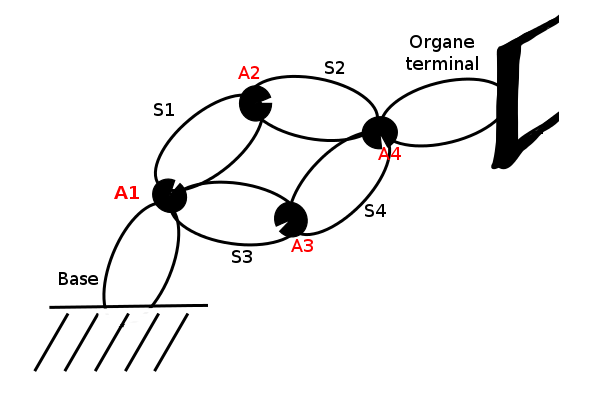
\includegraphics[width=.48\linewidth]{./chapter0/figures/closedchain.png}}
    \caption{\footnotesize{Exemples de cha\^ines cinématiques ouvertes et 
fermées : les $S_i$ représentent les différents segments intermédiaires, tandis 
que les $A_i$ correspondent aux articulations. Dans Fig.\ref{intro:fig1view0}, 
tous les segments $S_i$ ont un degré de connexion égal à 2 ; seuls la base et 
l'organe terminal ont un degré de connexion égal à 1. On peut voir au 
contraire dans Fig.\ref{intro:fig1view1} que tous les segments $S_i$ -- \`a 
l'exception donc de la base et de l'organe terminal -- possèdent un degré de 
connexion \'egal à 3.}}
\label{intro:fig1}
\end{figure}

\subsection{Architectures séries} \label{chap0-0-1}

{\it On appelle robot série un système constitué d'une chaîne cinématique 
ouverte dont chaque segment est relié au suivant par une articulation simple} 
(Fig.\ref{intro:fig2}). Longtemps dominants dans l'industrie, les robots séries 
ont été privilégiés grâce à un erelative simplicité de la commande et un espace 
de travail important.

\begin{figure}[!ht]
  \centering
      \subfloat[Robot série présentant 3 articulations 
rotoïdes]{\label{intro:fig2view0}
    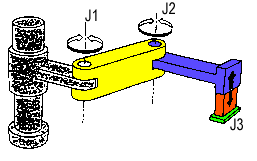
\includegraphics[width=.48\linewidth]{./chapter0/figures/serialrobot01.png}} 
\hfill
    \subfloat[Robot série présentant 3 articulations 
prismatiques]{\label{intro:fig2view1}
    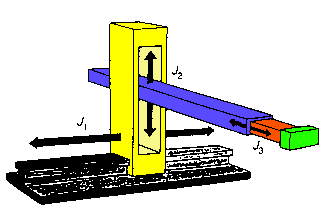
\includegraphics[width=.48\linewidth]{./chapter0/figures/serialrobot02.png}}
    \caption{\footnotesize{Exemples de robots séries (type SCARA et 
cart\'esien)}}
\label{intro:fig2}
\end{figure}

Une architecture série présente toutefois plusieurs inconvénients non 
négli\-gea\-bles dans un contexte industriel tels que :
\begin{itemize}
 \item chaque segment et articulation porte la charge de tous ceux qui leur 
succèdent dans la chaîne cinématique, ce qui pénalise la dynamique : segments 
et 
articulations doivent donc être rigidifiés et deviennent plus lourds, 
 \item les erreurs de positionnement se propagent de segments en segments ; la 
précision tout comme la répétabilité du manipulateur en sont affectées,
 \item les charges manipulables ne peuvent être \'elev\'ees, en raison des 
sollicitations en flexion sur les segments et de l'effet de bras de levier sur 
les premiers segments.
\end{itemize}

Ainsi, une architecture série impose souvent un dispositif imposant, dont la 
précision, la dynamique et la faible capacité de charges se révèleront 
insuffisants pour certaines tâches requises en particulier par l'industrie 
moderne.

Constitu\'ees de plusieurs cha\^ines cin\'ematiques ferm\'ees, les 
architectures parallèles pr\'sentent une alternative efficace aux limites des 
robots s\'eries.  Leurs caractéristiques, sur lesquel\-les nous allons \`a 
pr\'esent nous pencher, ont contribué à ce qu'elles s'installent 
progressivement 
dans le paysage de la robotique.

\subsection{Architectures parallèles} \label{chap0-0-2}

Une définition des robots parallèles est donnée dans \cite{merlet1997robots} :\\
{\it Un manipulateur parallèle est constitué d’un organe terminal à $n$ degrés 
de li\-berté et d’une base fixe, reliés entre eux par au moins deux chaînes
cinématiques indépendantes, la motorisation s’effectuant par $n$ actionneurs 
simples.}\\

Parmi les exemples les plus cités dans la littérature, nous trouvons 
la plate-forme de Gough-Stewart \cite{1956:Gough}, \cite{1965:Stewart} 
(Fig.\ref{intro:fig3view0},\ref{intro:fig3view1})et le 
robot Delta \cite{1988:Clavel} (Fig.\ref{intro:fig3view2}).

Initialement développée pour des applications li\'ees \`a l'industrie 
automobile (Fig.\ref{intro:fig3view0}), la plate-forme de Gough-Stewart a par 
la 
suite été utilisée dans des applications diverses parmi lesquelles les 
simulateurs de vols (Fig.\ref{intro:fig3view1}). Sa plate-forme mobile peut 
être déplacée selon 6 degrés de liberté (3 translations $+$ 3 rotations) à 
l'aide de six jambes indépendantes actionnées par des vérins pneumatiques. Les 
articulations la reliant à la base (cardan) et à la plate-forme (rotule) sont 
quant à elles laissées libres.

Le robot Delta (Fig.\ref{intro:fig3view2}) permet un déplacement de sa 
platforme 
selon les trois degrés de liberté de translation. Trois jambes sont utilisées 
pour cela, chacune étant reliée à la base par une articulation rotoïde à un 
levier, lui-même relié à un parallélogramme par une seconde articulation 
rotoïde, une troisième articulation rotoïde liant ce segment à l'organe 
terminal. Il peut atteindre des vitesses allant jusqu'à 10 m/s et des 
accélérations jusqu'à 20G, ce qui le rend particulièrement adapté pour des 
tâches de conditionnement. 

\begin{figure}[!ht]
  \centering
      \subfloat[Plateforme de Gough utilisée dans une usine de 
pneumatiques]{\label{intro:fig3view0}
    
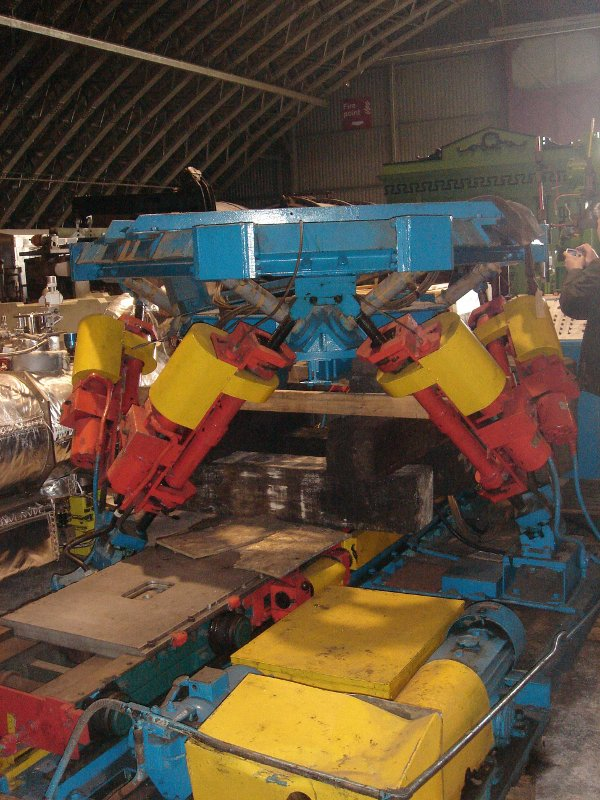
\includegraphics[width=.34\linewidth]{./chapter0/figures/parallelrobot01.jpg}} 
\hfill
    \subfloat[Plateforme de Gouch-Stewart utilisée pour des simulateurs de 
vols]{\label{intro:fig3view1}
    
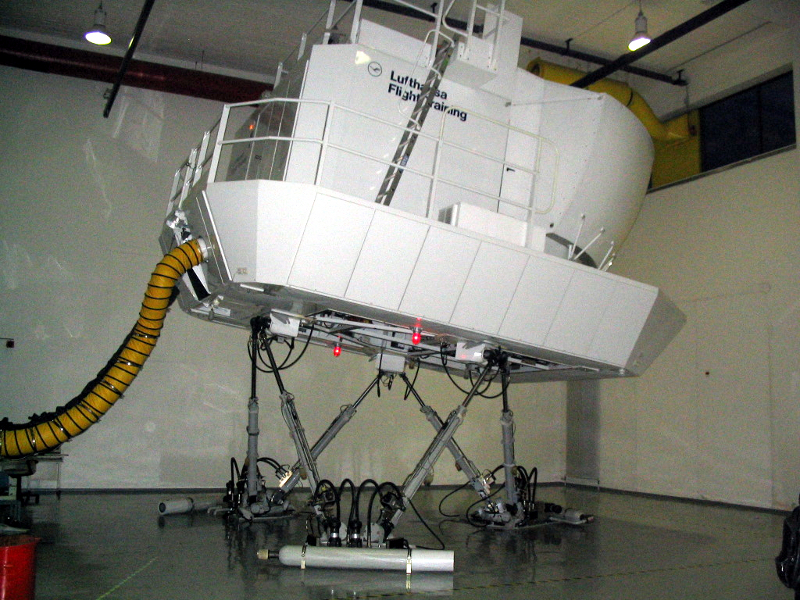
\includegraphics[width=.60\linewidth]{./chapter0/figures/parallelrobot02.jpg}} 
\\
    \subfloat[Robot Delta, particulièrement adapté aux tâches de 
conditionnement 
ou de ``pick and place'']{\label{intro:fig3view2}
    
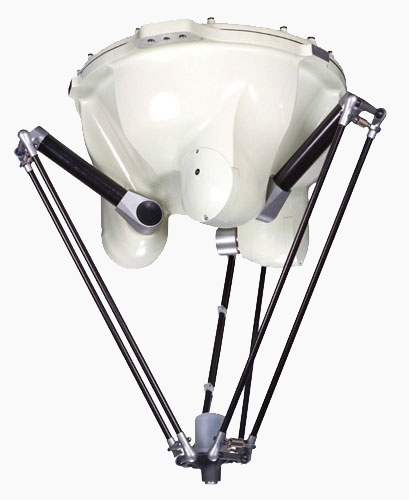
\includegraphics[width=.45\linewidth]{./chapter0/figures/parallelrobot03.jpg}}
    \caption{\footnotesize{Exemples de robots parallèles}}
\label{intro:fig3}
\end{figure}

De manière générale, les manipulateurs parallèles présentent les 
caractéristi\-ques sui\-vantes permettant de les comparer avantageusement aux 
manipulateurs séries :
\begin{itemize}
 \item une précision accrue par un mécanisme de {\bf compensation} des erreurs 
entre les différentes chaînes cinématiques (parfois appelées {\it jambes}),
 \item une capacité de charge élevée due à la {\bf répartition} de la charge 
sur 
les différentes jambes,
 \item une rigidité élevée car les éléments de chaînes sont sollicités en 
traction/compression plutôt qu'en flexion.
 \item une dynamique élevée conséquente de la {\bf coopération} des différentes 
jam\-bes dans le positionnement de l'organe terminal.
\end{itemize}

Toutefois, les mécanismes parallèles possèdent plusieurs inconvénients qui 
doivent être pris en compte lors du choix d'une architecture :
\begin{itemize}
 \item des relations complexes entre entrées et sorties,
 \item des positions dites {\it singulières} pouvant conduire à une perte de 
contrôle du manipulateur, et qui limite l'espace de travail.
 \item un espace de travail restreint par les limites de variation des 
variables articulaires. A titre d'exemple, la variation d'altitude d'une 
plate-forme de Gough-Stewart ne peut excéder la course des actionneurs 
linéaires des jambes.
\end{itemize}

L'architecture des robots parallèles à c\^ables que nous allons présenter dans 
la section suivante a été proposée dans le but de s'affranchir de la contrainte 
de limitation de l'espace de travail, qui est une contrainte forte des 
mécanismes parallèles \cite{journals/jfr/AlbusBD93}, 
\cite{1985:Landsberger.Sheridan*1}. L'intégralité des travaux présentés 
dans ce manuscrit étant consacré à l'étude et au développement de cette 
catégorie particulière de manipulateurs, nous utiliserons dorénavant pour les 
désigner les noms de robots, manipulateurs, robots parallèles à câbles ou CDPR 
(pour {\it cable-driven parallel robot}).

\section{Les manipulateurs parallèles à câbles} \label{chap0-1}

Les manipulateurs parallèles à câbles présentent une structure en chaînes 
cinéma\-tiques fermées, la base et la plate-forme étant reliées au moyen de 
câbles. Les actionneurs sont en général positionnés sur la base et leur 
fonction 
consiste à contrôler la longueur des câbles.

Afin de contrôler la longueur des câbles, plusieurs types de systèmes peuvent 
être utilisés, parmi lesquels :
\begin{itemize}
 \item un tambour actionné par un moteur rotatif sur lequel s'enroule ou se 
déroule le câble (Fig.\ref{intro:fig4view0}). La mesure de la longueur du câble 
déroulé est obtenue en mesurant la rotation du tambour ; cette mesure est 
relativement imprécise si l'enroulement n'est pas guidé.
 \item le câble est attaché au chariot d'un actionneur linéaire, un système de 
démultiplication à poulies permettant d'amplifier le déplacement du câble 
(Fig.\ref{intro:fig4view1}). La mesure du déplacement du chariot permet une 
estimation précise de la longueur du câble \cite{merlet2008}. 
\end{itemize}

\begin{figure}[!ht]
  \centering
      \subfloat[L'enroulement et le déroulement des câble se fait ici par un 
système de poulie actionnée par un moteur]{\label{intro:fig4view0}
    
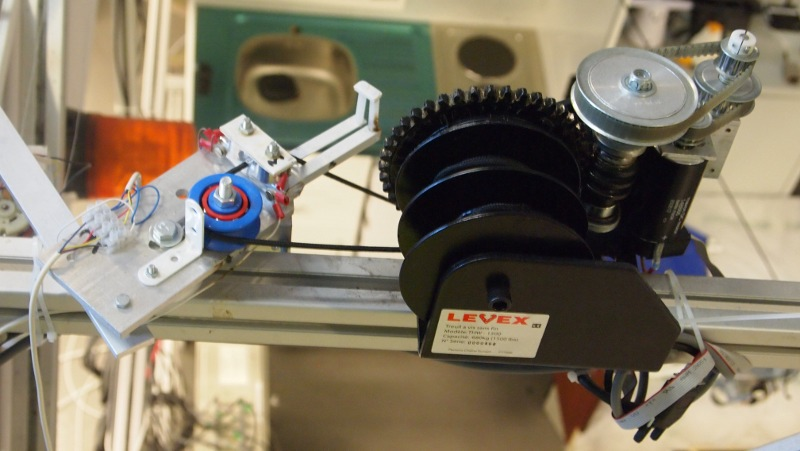
\includegraphics[width=.55\linewidth]{./chapter0/figures/winchesactuator.jpg}} 
\hfill
    \subfloat[Les câbles sont fixés à des plate-formes pouvant se déplacer 
linéairement sur des rails, permettant un contrôle de la 
longueur]{\label{intro:fig4view1}
    
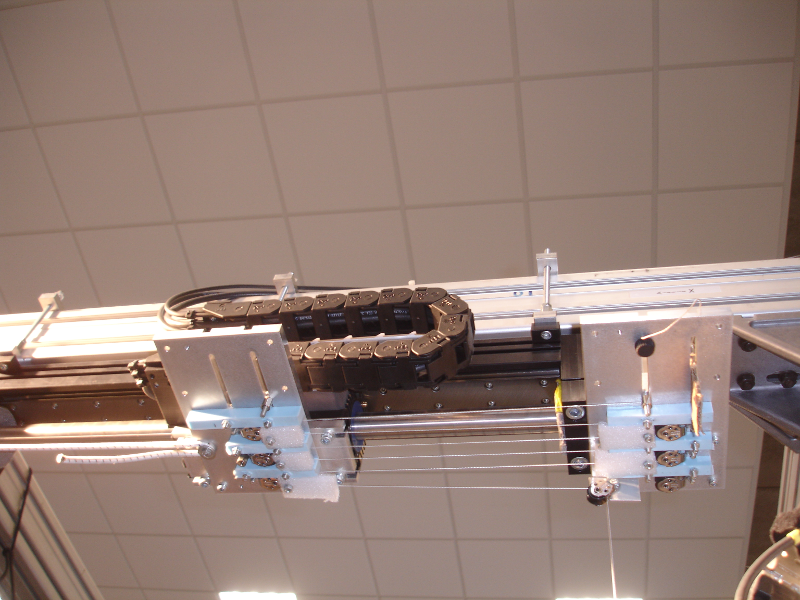
\includegraphics[width=.42\linewidth]{./chapter0/figures/linearactuator.png}}
    \caption{\footnotesize Deux types d'articulations et d'actionnement pour un 
robot à câble}
\label{intro:fig4}
\end{figure}

Dans tous les cas, ces systèmes permettent d'obtenir une très large variation 
sur les longueurs des câbles, solutionnant ainsi le problème de l'espace de 
travail. On a pu ainsi construire des robots travaillant sur des volumes de
$100m\times35m\times35m$ ({\tt Marionet-Crane}, \cite{merlet2010} 
Fig.\ref{intro:fig7view0}).

Toutefois, quelque-soit le type d'articulation et d'actionnement choisis, la 
force que peut exercer un seul câble sur l'organe terminal est nécessairement 
unilatérale : {\em un câble seul peut tirer, mais ne peut pas pousser la 
plate-forme}. Il faut donc, pour pouvoir contrôler le mouvement dans son 
intégralité, que les câbles subissent une opposition. Il a ainsi été montré que 
$n+1$ câbles au minimum sont requis pour assurer le contrôle de $n$ degrés de 
liberté \cite{1994:Ming.Higuchi}. On peut cependant considérer la gravité comme 
une force unilatérale et la représenter comme un câble virtuel jouant le rôle 
d'opposition : il est ainsi possible de n'utiliser que $n$ câbles pour $n$ 
degrés de liberté.

On distingue donc deux types de configurations pour un robot parallèle à câbles 
:
\begin{itemize}
 \item en {\it configuration suspendue} (Fig.\ref{intro:fig5view1}), la gravité 
agit comme un câble virtuel : les câbles sont fixés généralement au point le 
plus haut du dispositif, et $n$ suffisent pour déplacer et orienter l'organe 
terminal selon $n$ degrés de liberté. On retrouve parfois ce type de 
configuration dans la littérature sous le nom de {\it grue}/{\it crane}. A 
titre d'exemple, le manipulateur {\it Nist Spider} 
\cite{1992:Albus.Bostelman.ea} présente une configuration suspendue.
 \item en {\it configuration pleinement contrainte} 
(Fig.\ref{intro:fig5view0}), 
les câbles travaillent en opposition et $n+1$ sont nécessaires pour assurer des 
déplacements et l'application de forces correspondant à $n$ degrés de liberté.
\end{itemize}

\begin{figure}[!ht]
  \centering
     \subfloat[Exemple de configuration pleinement 
contrainte]{\label{intro:fig5view0}

\includegraphics[width=.50\linewidth]
{./chapter0/figures/robot_cdpr_noncrane.jpg}} 
\hfill
    \subfloat[Exemple de configuration suspendue]{\label{intro:fig5view1}
    
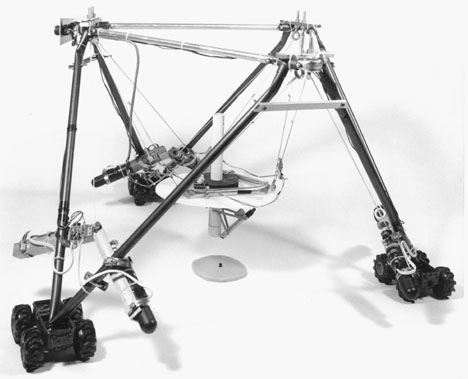
\includegraphics[width=.40\linewidth]{./chapter0/figures/robot_cdpr_crane.jpg}}
    \caption{\footnotesize Deux configurations possibles pour un robot 
parallèle 
à câble}
\label{intro:fig5}
\end{figure}

Une caractéristique particulière des manipulateurs parallèles à câbles qui les 
différencie des manipulateurs parallèles classiques est la {\bf non-rigidité 
des 
jam\-bes}. Sous certaines conditions, un ou plusieurs câbles peuvent être 
détendus, ce qui a pour effet qu'ils n'exercent plus de force sur la 
plate-forme. Nous reviendrons plus loin sur ce point essentiel.

Comparativement donc aux robots parallèles classiques, les robots parallèles à 
câbles présentent les caractéristiques suivantes :
\begin{itemize}
 \item la structure parallèle permet de conserver les propriétés de 
compensation 
des erreurs, de répartition des charges et des efforts, de coopération des 
chaînes cinématique pour l'exécution d'un mouvement
 \item l'espace de travail est considérablement agrandi par rapport aux robots 
parallèles à jambes rigides
 \item l'équipage mobile est très léger, ce qui favorise la dynamique
 \item le comportement des câbles (non-déformables, élastiques, pesants, \dots) 
peut complexifier s\'erieusement le modèle du robot
 \item l'unilatéralité des forces implique que nous puissions nous retrouver 
dans une situation avec un ou plusieurs câbles détendus, ce qui doit être pris 
en compte dans le contrôle.
\end{itemize}

Après avoir introduit quelques notations, nous allons à présent décrire les 
modèles géométriques direct et inverse, cinématiques ainsi que l'équilibre 
statique pour les robots parallèles à câble. Ceci nous permettra de lister tant 
que faire se peut l'ensemble des difficultés posées par ce type de manipulateur 
et auxquelles nous avons été confrontées dans le cadre de nos recherches.

\subsection{Notations} \label{chap0-1-0}

\begin{figure}[!ht]
\centering
\def\svgwidth{.85\linewidth}
\input{./chapter0/figures/notation_schema.pdf_tex}
\end{figure}

\begin{itemize}
 \item $R_b$ : référentiel de la base
 \item $R_e$ : référentiel de l'organe terminal
 \item $A_i$ : point d'attache du $i^{\hbox{ème}}$ câble à la base ; le terme 
de 
{\it point de sortie} sera également utilisé.
 \item $B_i$ : point d'attache du $i^{\hbox{ème}}$ câble à l'organe terminal
 \item $C$ : un point arbitraire de l'organe terminal utilisé comme référence 
pour sa position
 \item $\rho_i$ : longueur réelle du câble $i$
 \item $l_i$ : longueur déroulée du câble $i$
 \item $\boldmath {\mathcal F}$ : vecteur des forces exercées sur l'organe 
terminal
 \item $\bf J$ : jacobienne du robot
\end{itemize}
Enfin, on utilisera la notation ${\bf J}^{-1}$ pour exprimer la jacobienne 
inverse, et ${\bf J}^{-T}$ sera utilisé comme raccourci de notation pour sa 
transposée.

Sauf mention du contraire, {\bf nous supposerons dans la suite que les câbles 
sont non-pesants et non-élastiques}, ce qui est une hypothèse adéquate pour le 
robot que nous avons utilisé.

\subsection{Modèle géométrique inverse} \label{chap0-1-1}

Le modèle géométrique inverse consiste à déterminer les coordonnées 
articulaires 
à partir des coordonnées opérationnelles. Dans le cas des robots parallèles à 
câbles, les coordonnées articulaires correspondent aux longueurs $\rho$ des 
câbles. Lorsque ceux-ci sont tendus, cette longueur doit être égale à la 
distance entre les points de sortie ${\bf A}_i$ et le point d'attache à la 
plate-forme ${\bf B}_i$. Dans le cas où le câble est détendu, la longueur sera 
supérieure à cette distance (Fig.\ref{intro:fig6view0}).\\

%%%%%% une figure différente
\begin{figure}[!ht]
  \centering
      \subfloat[Forme d'un câble dont la tension serait 
nulle]{\label{intro:fig6view0}
    
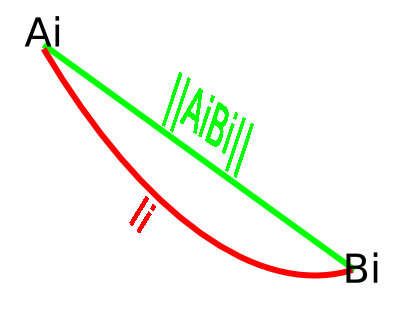
\includegraphics[width=.35\linewidth]{./chapter0/figures/nulltensionwire.png}} 
\hfill
    \subfloat[Câble élastique sur lequel est appliquée une tension positive : 
la 
longueur réelle diffère de la longueur déroulée]{\label{intro:fig6view1}
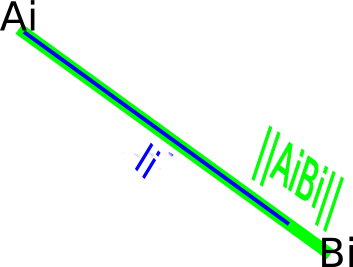
\includegraphics[width=.35\linewidth]
{./chapter0/figures/positivetensionwire.png}}
    \caption{\footnotesize{Dans le cas d'un câble détendu (tension nulle), la 
longueur déroulée sera supérieure à la distance entre les deux points d'attache 
; de plus, la forme du câble sera telle qu'il y a risque d'intersection avec 
d'autres câbles, l'environnement, \dots. Dans le cas d'un câble élastique tendu 
(tension strictement positive), la longueur déroulée $l_i$ sera inférieure à la 
distance entre les points d'attache correspondant à la longueur réelle du 
câble $\rho_i$}}
\label{intro:fig6}
\end{figure}

Nous partons donc des relations suivantes :
\begin{eqnarray}
\rho_i &=& ||{\bf A}_i {\bf B}_i||, \hbox{ si } \tau_i > 0 \\ 
\rho_i &\geq& ||{\bf A}_i {\bf B}_i||, \hbox{ si } \tau_i = 0
\label{intro:eq1}
\end{eqnarray}

Comme on le voit, il n'est pas possible d'obtenir les longueurs $\rho_i$ sans 
prendre en compte les tensions $\tau_i$. Dès lors, tout comme dans l'approche 
développée par \cite{2010:Carricato.Merlet}, nous parlerons donc de modèle 
géométrico-statique inverse, requérant l'étude de l'équilibre statique.

\subsection{Equilibre statique} \label{chap0-1-2}

On dit d'un solide au repos qu'il est en équilibre statique lorsque l'ensemble 
des forces extérieures $\mathcal {\bf F}_{\hbox{ext}_i}$ qui s'exercent sur lui 
s'annulent, ce qui se traduit par la relation suivante :
\begin{equation}
\sum_i \boldmath {\mathcal F}_{\hbox{ext}_i} = {\bf 0}
\label{intro:eq2}
\end{equation}

Sous l'hypothèse que les forces mécaniques de frottement et de résistance 
peuvent être ici négligées, nous considérons uniquement la force de gravité 
exercée sur la plate-forme ainsi que les efforts exercés par chacun des câbles.

La direction dans laquelle un câble de longueur $\rho_i$ relié à la base au 
point ${\bf A}_i$ et à la plate-forme au point ${\bf B}_i$ exerce une force sur 
la plate-forme est donnée par le vecteur ${\bf u}_i = \frac{{\bf A}_i{\bf 
B}_i}{\rho_i}$. On peut dès lors définir pour ce câble un torseur ${\bf W}_i$ 
correspondant aux efforts et couples exercés par celui-ci sur la plate-forme :
\begin{equation}
{\bf W}_i = -({\bf u}_i^T, (p_i \times {\bf u}_i)^T)^T
\label{intro:eq3}
\end{equation}
où $p_i$ est un vecteur allant d'un premier point de référence arbitraire 
$C$ localisé sur la plate-forme au point ${\bf B}_i$. La force exercée par le 
câble sur la plate-forme est alors $ \tau_i {\bf W}_i$ , où $\tau_i$ est un 
scalaire positif représentant l'intensité de la tension.

Soit ${\bf W}_g$ le torseur indiquant la direction dans laquelle la gravité est 
exercée dans le référentiel choisi, pour $n$ câbles, (Equ.\ref{intro:eq2}) 
s'écrit pour nous :
\begin{equation}
\begin{bmatrix}
 {\bf W}_1 & {\bf W}_2 & \dots & {\bf W}_n & {\bf W}_g
\end{bmatrix}
\begin{bmatrix}
 \tau_1 \\ \tau_2 \\ \dots \\ \tau_n \\ \hbox{mg}
\end{bmatrix}
= {\bf 0}
\label{intro:eq4}
\end{equation}

En posant ${\bf \tau} = (\tau_1, \tau_2, \dots, \tau_n)^T$, ${\bf W}$ la 
matrice 
$6 \times n$ dont les colonnes sont les $n$ torseurs ${\bf W}_i$, et en isolant 
$\mathcal {\bf F} =  \hbox{mg} {\bf W}_g$ modélisant la force de gravité, la 
relation (Equ.\ref{intro:eq4}) s'écrit également :
\begin{equation}
\mathcal {\bf F} + {\bf W} \tau = {\bf 0}
\label{intro:eq5a}
\end{equation}

soit  
\begin{equation}
\mathcal {\bf F} = {\bf J}^{-T} {\bf \tau}
\label{intro:eq5b}
\end{equation}
où ${\bf J}^{-1} = - {\bf W}^T$ est une matrice que l'on appelle {\it 
jacobienne 
inverse}.

\subsection{Modèle géométrico-statique inverse (ou {\it MGSI})} 
\label{chap0-1-3}


Connaissant les paramètres de pose de la plate-forme, on veut en déduire les 
longueurs supposées $\rho_i$ des câbles : c'est le modèle géométrique inverse. 
Dans le cas où nous avons $m \geq 6$ câbles, connaissant la pose 
${\bf B}$ et les points de sorties ${\bf A}_i$, on peut calculer les longueurs 
$\rho_i$. Si $m = 6$, la solution de l'équilibre statique est unique, 
l'\'equilibre statique possède sinon en théorie une infinité de solution (nous 
ne devons toutefois consid\'erer que les ensembles de solutions pour lesquelles 
les $\tau_i$ sont tous strictement positifs).

Il est cependant n\'ecessaire d'envisager les possibilit\'es pour lesquelles 
moins de $6$ c\^ables sont en tension. Nous avons d\`es lors $m < 6$, et nous 
ne pouvons donc plus sp\'ecifier que $m$ degr\'es de libert\'es : il faut alors 
faire intervenir la statique afin de calculer les $6-m$ degr\'es de libert\'e. 
Plusieurs m\'ethodes s'offrent \`a nous, dont :
\begin{itemize}
 \item par r\'esolution inverse de l'\'equilibre statique, on \'elimine les 
$\tau$ correspondant aux c\^ables mous, puis on reporte dans les \'equations du 
mod\`ele g\'eom\'etrique inverse, ce qui nous donne $6-m$ \'equations.
\item L'équilibre statique est vérifié 
uniquement si l'ensemble des déterminants $m+1 \times m+1$ de la matrice ${\bf 
W}$ sont nuls \cite{carricato_merlet2013}. Si tous les $\tau_i$ sont 
strictement positifs, le modèle géométrico-statique possède alors une solution, 
mais correspondant à un mode dégradé du système.
\end{itemize}


\subsection{Modèle géométrico-statique direct}\label{chap0-1-4}

Résoudre le modèle géométrique direct consiste à calculer les coordonnées 
opéra\-tionnelles à partir de la donnée des coordonnées articulaires. Il s'agit 
donc dans le contexte d'un robot parallèles à câbles de déduire la pose de la 
plate-forme (position et orientation) à partir des longueurs des câbles. C'est 
un problème qui a posé de nombreux défis mathématiques et algorithmiques dans 
le 
cas des robots parallèles rigides \cite{merlet1997robots}, et nous allons voir 
qu'il peut \^etre plus complexe dans le cas des CDPR.

On distinguera les cas suivants :
\begin{itemize}
  \item $m > 6$ : dans le cas o\`u nous avons $m > 6$ c\^ables, les inconnues 
sont les $6$ param\`etres de pose de $\bf X$. Nous avons $6 > m$ \'equations 
fournies par le mod\`ele g\'eom\'etrique. Le syst\`eme \`a r\'esoudre ne 
poss\`ede cependant en g\'en\'eral aucune solution : on en d\'eduit alors qu'un 
ou plusieurs c\^ables sont mous, ce que l'\'etude de l'\'equilibre statique 
nous permettront de v\'erifier. On cherche alors les solutions valides pour 
$m-1$ c\^ables.
  \item $m = 6$ : cette situation peut \^etre ramen\'ee \`a son 
\'equivalent pour les robots parall\`eles classiques ; dans ce cas, les 
\'equations g\'eom\'etriques et celles de la statique sont d\'ecoupl\'ees. La 
g\'eom\'etrie nous donne les poses $\bf X$, et on v\'erifie la validit\'e de 
celles-ci avec la statique.
  \item $m < 6$ : ici, nous avons $6$ inconnues (les param\`etres de pose $\bf 
X$). Or, le mod\`ele g\'eom\'etrique ne fournit que $m < 6$ \'equations. On 
compl\`etera d\`es lors le syst\`eme avec les \'equations de l'\'equiibre 
statique. Dans cette nouvelle situation, nous avons $6 + m$ inconnues ($6$ 
param\`etres de pose et $m$ tensions) pour $6 + m$ \'equations (dont $m$ sont 
fournies par le mod\`ele g\'eom\'etrique et $m$ par l'\'equilibre statique). On 
obtient alors bien un syst\`eme carr\'e, mais dont le nombre d\'equations est 
tr\`es sup\'erieur \`a son \'equivalent pour les robots parall\`eles \`a jambes 
rigides. Dans le cas $m = 5$, on a en effet $11$ \'equations pour les robots 
parall\`eles \`a c\^ables, contre $5$ pour les robots parall\`eles rigides.
Toutefois, le syst\`eme de $n+6$ \'equations \`a $n+6$ inconnues ainsi obtenu 
n'est valide qu'`a la condition que tous les c\^ables soient tendus, soit que 
$\forall i \in [0,m], \rho_i = ||{\bf A}_i{\bf B}_i||$. On ne peut jamais 
exclure que la plate-forme soit dans une pose pour laquelle $\exists i \in 
[1,m], \rho_i > ||{\bf A}_i{\bf B}_i||$. Dans ce cas, une des \'equations du 
mod\`ele g\'eom\'etrique ne sera plus valide. Il faut donc consid\'erer tous 
les cas avec $6+m-p$ \'equations ($p \in [1, m-1]$) et v\'erifier $p$ fois la 
validit\'e des r\'esultats ($\rho_i > ||{\bf A}_i{\bf B}_i||$, $\tau_i > 0$). 
\end{itemize}

Ce qui doit \^etre retenu ici est qu'il est difficile lors d'un déplacement de 
prévoir à l'avance quels câbles seront en tension en chaque point de la 
trajectoire ainsi que la valeur des tensions.

Ce point, très peu mentionné dans la littérature, est un des inconvénients 
majeurs de l'utilisation des robots parallèles à câbles. Le premier chapitre de 
ce travail montrera qu'il est toutefois possible d'élaborer une stratégie 
prenant ce problème en compte pour améliorer le contrôle et la stabilité du 
système pour la grande majorité des situations.

\subsection{Modèle cinématique}\label{chap0-1-5}

Le modèle cinématique consiste à établir une relation entre les 
vitesses articulaires ${\bf \dot \Theta}$ et la vitesse (translation et 
angulaire) de la plate-forme $\bf \Omega$.

Nous avons vu que le vecteur ${\bf A}_i{\bf B}_i$ peut être calculé de deux 
manières différentes :
\begin{itemize}
 \item connaissant la pose de la plate-forme et sa géométrie, les coordonnées 
de 
${\bf B}_i$ sont données ; ${\bf A}_i$ étant connu par la géométrie du robot, 
on 
peut définir une fonction $H_1$ dépendante uniquement de la pose telle que :
\begin{equation}
{\bf A}_i{\bf B}_i = H_{1_{|i}}({\bf X})
\label{intro:eq6}
\end{equation}
 \item à partir des coordonnées articulaires (et éventuellement de la pose si 
l'intervention de l'équilibre statique est requise), le {\it MGSD} permet de 
définir la relation suivante :
\begin{equation}
{\bf A}_i{\bf B}_i = H_{2_{|i}}({\bf X}, {\bf \Theta})
\label{intro:eq7}
\end{equation}
\end{itemize}
 
Si ${\bf AB}$ est le vecteur composé des différents ${\bf A}_i{\bf B}_i$, alors 
on obtient en combinant (Equ.\ref{intro:eq6}) et (Equ.\ref{intro:eq7}) :
\begin{equation}
\begin{matrix}
{\bf AB} &=& H_1({\bf X}) \\
{\bf AB} &=& H_2({\bf X}, {\bf \Theta}) \\
\Longrightarrow & & H_1({\bf X}) = H_2({\bf X}, {\bf \Theta})
\end{matrix}
\label{intro:eq8}
\end{equation}

En différentiant (Equ.\ref{intro:eq8}), on obtient :
\begin{equation}
\frac{\partial H_1}{\partial {\bf X}} \frac{\partial {\bf X}}{\partial {\bf t}} 
=  \frac{\partial H_2}{\partial {\bf X}} \frac{\partial {\bf X}}{\partial {\bf 
t}} + \frac{\partial H_2}{\partial {\bf \Theta}} \frac{\partial {\bf 
\Theta}}{\partial {\bf t}}
\label{intro:eq9}
\end{equation}

soit :

\begin{equation}
\dot {\bf \Theta} = \left ( \frac{\partial H_2}{\partial {\bf \Theta}} \right 
)^{-1} \left (\frac{\partial H_1}{\partial {\bf X}} - \frac{\partial 
H_2}{\partial {\bf X}} \right ) \dot {\bf X}
\label{intro:eq10}
\end{equation}

Si $\left ( \frac{\partial H_2}{\partial {\bf \Theta}} \right )$ est bien 
inversible, nous pouvons définir une matrice $J^{-1}$ de manière à obtenir la 
relation suivante :
\begin{equation}
\dot {\bf \Theta} = J^{-1} \dot {\bf X}
\label{intro:eq11}
\end{equation}

Toutefois, le vecteur $\dot {\bf X}$ ainsi d\'etermin\'e ne correspond pas \`a 
$\bf \Omega$, il d\'epend de la param\'etrisation choisie pour les param\`etres 
de pose. En particulier, si nous utilisons les angles d'Euler pour param\'etrer 
l'orientation de la plate-forme, nous pouvons exprimer la v\'elocit\'e d'un 
point ${\bf B}$ en fonction de la vitesse d'un point ${\bf C}$ de r\'ef\'erence 
de la plate-forme avec la relation suivante :
\begin{equation}
{\bf v_B} = {\bf v_C} + {\bf BC} \times {\bf \omega_c}
\label{intro:eq11b}
\end{equation}
o\`u $\bf V_C$ d\'enote la v\'elocit\'e de la plate-forme au point ${\bf C}$, 
et ${\bf \omega_C}$ le vecteur des v\'elocit\'es angulaires.

Ainsi, comme ${\bf A}_i$ est fix\'e, nous avons pour le c\^able $i$ :
\begin{equation}
\dot { {\bf A}_i{\bf B}_i } = {\bf v_C} + {\bf B}_i{\bf C} \times {\bf \omega_c}
\label{intro:eq11c}
\end{equation}

En posant :
\begin{equation}
\dot {\bf X} = \begin{matrix}
                {\bf V_C} \\
		{\bf \omega_C}
               \end{matrix}
\label{intro:eq11d}
\end{equation}
nous construisons ainsi une relation entre les vitesses articulaires et les 
vitesses de translation et d'orientation, ces derni\`eres param\'etr\'ees par 
les angles d'Euler.

La matrice $J^{-1}$ ainsi construite est appelée {\it Jacobienne 
inverse param\'etr\'e} par les angles d'Euler. On notera qu'elle dépend à la 
fois des paramètres de pose et des coordonnées articulaires : il requiert d\`es 
lors la r\'esolution des mod\`ele g\'eom\'etriques direct et inverse.

\section{Les robots N-1} \label{chap0-2}

On parle de configuration N-1 pour un robot parall\`ele \`a c\^ables en 
configuration suspendue lorsque l'ensemble des c\^ables sont reli\'es \`a la 
plate-forme en un m\^eme point ${\bf B}$. Cette architecture pr\'esente les 
caract\'eristiques suivantes :
\begin{itemize}
  \item puisque l'ensemble des points ${\bf B}_i$ sont confondus, le contr\^ole 
en orientation n'est plus possible : c'est donc une architecture d\'edi\'ee aux 
d\'eplacements en translation. Entre autres avantages, nous n'avons plus \`a 
nous pr\'eoccuper des inerf\'erences entre c\^ables.
  \item si $N > 3$, seuls trois c\^ables au plus seront en tension positive et 
permettront de contr\^oler les d\'eplacements de la plate-forme ; le cas N-4 
sera expliqu\'e en d'etail \`a l'occasion du chapitre consacr\'e aux 
configurations de c\^ables.
  \item les tensions n'\'etant r\'eparties qu'entre au plus trois c\^ables, 
l'ajout de c\^ables suppl\'ementaires ne peut servir \`a soulager les autres 
c\^ables. Par contre, il est possible d'envisager de choisir le meilleur 
triplet 
en fonction d'un crit\`ere donn\'e, parmi tous ceux que l'utilisation de $N>3$ 
c\^ables rend possible ($4$ triplets au plus pour $4$ c\^ables, $10$ pour $5$ 
c\^ables, $20$ pour $6$ c\^ables, $\cdots$). De plus, l'utilisation de c\^ables 
suppl\'ementaires permet d'augmenter l'espace de travail du robot, lorsque le 
point d'attache du c\^able ajout\'e est plac\'e en dehors de celui-ci.
\end{itemize}

\subsection{Mod\`eles g\'eom\'etriques}

{\bf MGSD :}\\

\begin{figure}[!ht]
  \centering
    \def\svgwidth{.85\linewidth}
      \input{./chapter0/figures/MGDN1.pdf_tex}
    \caption{\footnotesize{Repr\'esentation des points d'intersection des 
trois sph\`eres de centre ${\bf A}_i$ (resp. ${\bf A}_j$, ${\bf A}_k$) et de 
rayon $\rho_i$ (resp. $\rho_j$, $\rho_k$). Dans ce cas pr\'ecis, la solution la 
plus haute est haut-dessus du plan contenant les points ${\bf A}_i$, ${\bf 
A}_j$ et ${\bf A}_k$ : elle ne peut se retrouver en \'equilibre statique, 
aucun c\^able ne pouvant fournir une force oppos\'ee \`a la force de 
gravit\'e.}}
\label{intro:fig6b}
\end{figure}

Soient $N$ c\^ables dont nous connaissons les longueurs $\rho_0, \cdots, 
\rho_{N-1}$. Puisque nous n'avons que $3$ c\^ables au plus en tension, nous 
commen\c cons par r\'esoudre le mod\`ele g\'eom\'etrique pour chaque 
triplet de c\^ables. Ne contr\^olant pas les rotations, les param\`etres de 
pose sont uniquementles coordonn\'ees dans l'espace. D\`es lors, nous avons $3$ 
inconnues, et $3$ \'equations. Les solutions fournies par la r\'esolution du 
syst\`eme seront ensuite valid\'ees par l'\'etude de l'\'equilibre statique. 
S'agissant des points d'intersections de trois sph\`eres de centre ${\bf A}_i$ 
et de rayon $\rho_i$, il y aura au maximum deux solutions pour chaque triplet 
de c\^ables, dont une au moins ne respectera pas l\'equilibre statique. Il y a 
donc pour chaque triplet de c\^ables au plus une pose valide \ref{intro:fig6b}.

Il faut ensuite v\'erifier que nous n'ayons pas une pose valide avec moins de 
$3$ c\^ables en tension : dans ce cas, nous avons deux \'equations donn\'ees 
par la g\'eom\'etrique, pour les trois inconnues que constituent les 
param\`etres de poses. En compl'etant avec la statique qui nous donne 3 
\'equations pour deux inconnues qui sont les tensions dans les deux c\^ables 
test\'es. Toutefois, les trois \'equations de la statique seront lin\'eairement 
d\'ependante. On ajoutera donc une derni\`ere \'equation de contrainte 
stipulant que la pose doit se trouver sur la projection verticale de la droite 
issue des points ${\bf A}_i$ et ${\bf A}_j$ test\'es. On proc\`edera enfin de 
m\^eme pour l'\'etude des cas \`a un seul c\^able en tension positive. \\


{\bf MGSI :}\\

Le mod\`ele g\'eom\'etric0-statique indirect est relativement simple dans ce 
contexte. Connaissant les param\`etres de pose, les longueurs de c\^ables 
peuvent \^etre imm\'ediatement d\'eduite \`a partir de la relation 

\begin{equation}
\rho_i = ||{\bf A}_iB||^2
\label{intro:eq11a}
\end{equation}

La solution ainsi d\'etermin\'ee est unique du point de vue de sa localisation 
dans l'espace, mais peut correspondre \`a plusieurs situations de triplets de 
c\^ables en tension.\\

{\bf Cin\'ematique :}\\

Si nous d\'erivons la relation pr\'ec\'edente \ref{intro:eq11a}, nous avons :
\begin{equation}
2 \rho_i \partial \rho = 2 x \partial x + 2 y \partial y + 2 z \partial z
\label{intro:eq11a2}
\end{equation}
avec ${\bf A}_i{\bf B} = {\bf X}_i = (x, y, z)$.

D\`es lors, on obtient :
\begin{equation}
\partial \rho = \frac x \rho \partial x + \frac y \rho \partial y + \frac y 
\rho \partial z
\label{intro:eq11a3}
\end{equation}

On en d\'eduira pour le c\^able $i$ la ligne correspondante de la 
Jacobienne inverse :
\begin{equation}
{\bf J}^{-1}_i = 
\begin{bmatrix}
\frac {{\bf B}_x - {\bf A}_{i_x}} {\rho_i} & \frac {{\bf B}_y - {\bf A}_{i_y}} 
{\rho_i} & \frac {{\bf B}_z - {\bf A}_{i_z}} {\rho_i} 
\end{bmatrix}
\label{intro:eq11a4}
\end{equation}



\subsection{{\tt Marionet-Assist}} \label{chap0-2-2}

Les {\tt Marionet} sont une classe de robots à câbles développés par l'EPI 
Hephaistos pour des applications diverses \cite{merlet2010marionet} :
\begin{itemize}
 \item {\tt Marionet-Crane} (Fig.\ref{intro:fig7view0}) : intervention à grande 
échelle pour des opé\-rations de sauvetage dans des situations de catastrophe 
naturelle
 \item {\tt Marionet-VR} (Fig.\ref{intro:fig7view1}) : utilisation en dans des 
environnements de r\'ealit\'e virtuel en tant que g\'en'erateur de mouvement et 
comme interface haptique. 
 \item {\tt Marionet-Rehab} (Fig.\ref{intro:fig7view2}) : rééducation et 
assistance à la personne ; pouvant atteindre des vitesses allant jusqu'à 
100m/s, 
il est également possible de l'utiliser pour des opérations de transfert 
ultra-rapides
 \item {\tt Marionet-School} (Fig.\ref{intro:fig7view3}) : pédagogie et 
diffusion ; ces robots sont utilisés entre autres pour illustrer de manière 
ludique des propriétés géométriques et mathématiques auprès des publics jeunes
\end{itemize}

\begin{figure}[!ht]
  \centering
    \subfloat[{\tt Marionet-Crane} : son espace de 
travail peut aller jusqu\`a $15m \times 15m \times 
15m$, et la l\'eg\`eret\'e de son \'equipement garantit 
un d\'eploiement rapide]{\label{intro:fig7view0}
    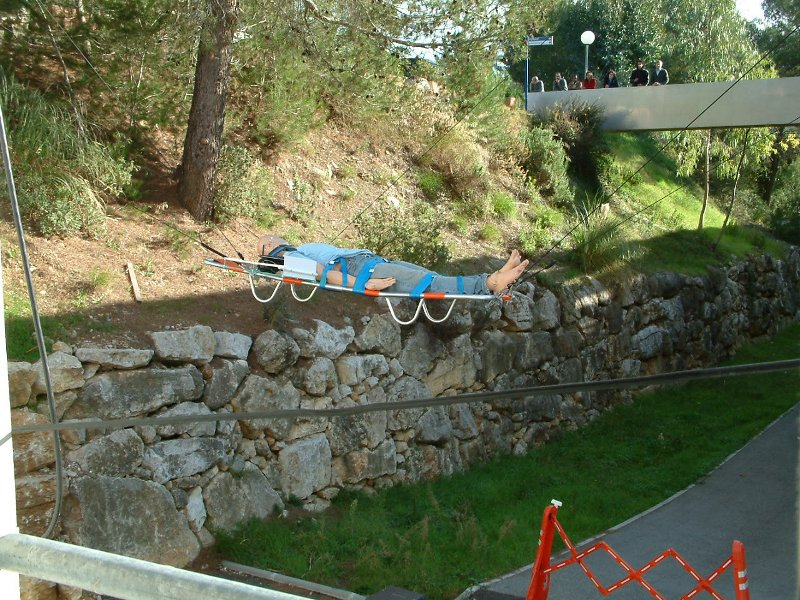
\includegraphics[width=.42\linewidth]{./chapter0/figures/marionet03.jpg}}  
\hfill
    \subfloat[{\tt Marionet-VR} : utilise des 
actionneurs lin\'eaires pour une pr\'ecision accrue 
dans un espace de travail de $6m \times 5m \times 
3m$]{\label{intro:fig7view1}
    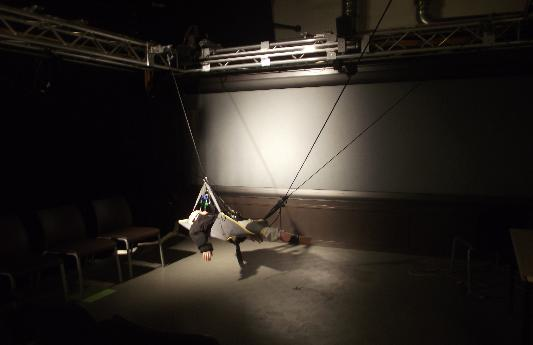
\includegraphics[width=.48\linewidth]{./chapter0/figures/marionet05.jpg}} \\
    \subfloat[{\tt Marionet-Rehab} : utilise des actionneurs lin\'eaires pour 
de la mesure de mouvements (mode passif) et des t\^aches de 
r\'ehabilitation (mode actif)]{\label{intro:fig7view2}
    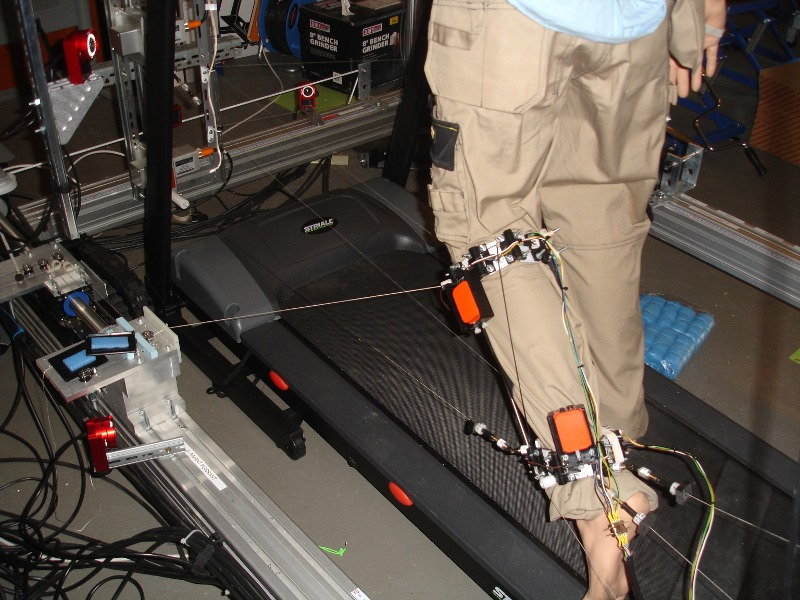
\includegraphics[width=.45\linewidth]{./chapter0/figures/marionet01.jpg}} 
\hfill
    \subfloat[{\tt Marionet-School} : ais\'ement 
transportable et d\'eployable, il est utilis\'e pour des interventions 
p\'edagogiques]{\label{intro:fig7view3}
    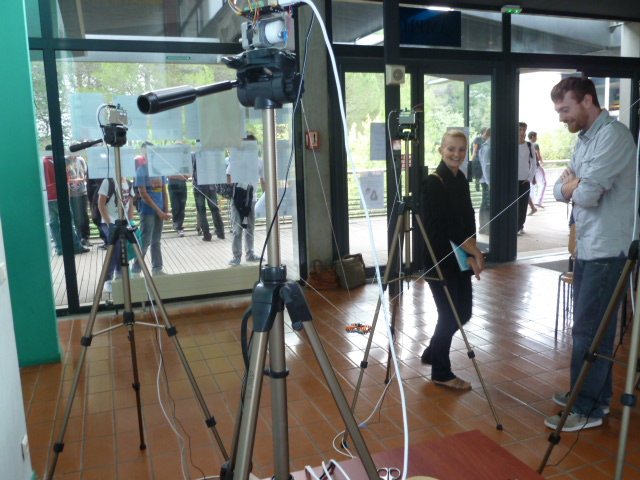
\includegraphics[width=.45\linewidth]{./chapter0/figures/marionet02.jpg}}
    \caption{\footnotesize{Exemples d'utilisation des robots {\tt Marionet}}}
\label{intro:fig7}
\end{figure}

Le robot {\tt Marionet-Assist} a été développé dans un objectif d'assistance 
aux 
personnes à mobilités réduites, et plus spécifiquement dans une démarche 
d'amélio\-ration de l'autonomie des publics concernés. Il doit pouvoir répondre 
à des situations tout aussi diverses que :
\begin{itemize}
 \item soutien ponctuelle au déplacement pour une personne âgée expérimentant 
une fatigue articulaire (par exemple pour la passage de la baignoire) 
(Fig.\ref{intro:fig8view0})
 \item aide au transfert d'une position à une autre pour une personne (des 
toilettes au fauteuil par exemple) 
(Fig.\ref{intro:fig8view1})
 \item aide aux aidants pour le transfert de personnes atteintes de 
tétraplégie (déplacement du lit vers un fauteuil par exemple) afin de r\'eduire 
la p\'enibilit\'e de leur t\^ache. 
(Fig.\ref{intro:fig8view2})
\end{itemize}

\begin{figure}[htp]
  \centering
  \subfloat[Simple soutien au déplacement dans une pièce de 
vie]{\label{intro:fig8view0}
  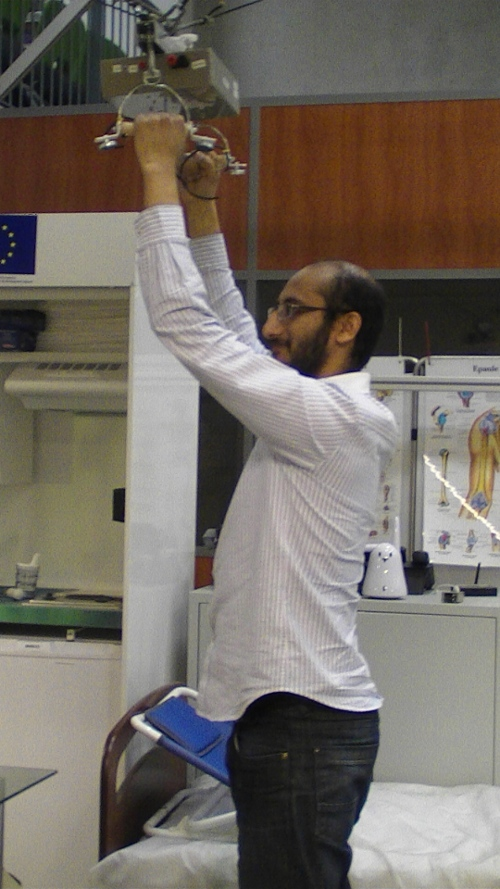
\includegraphics[width=.2\linewidth]{./chapter0/figures/case01.jpg}} \hfill
  \subfloat[Transfert de position assise/levé]{\label{intro:fig8view1}
  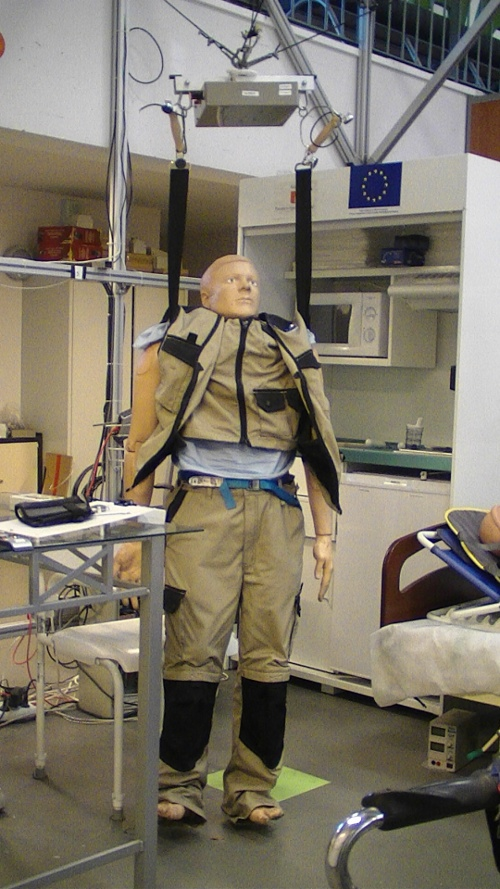
\includegraphics[width=.2\linewidth]{./chapter0/figures/case02.jpg}} \hfill
  \subfloat[Déplacement autonome d'un lieu de vie (lit) vers un dispositif de 
déplacement (fauteuil)]{\label{intro:fig8view2}
  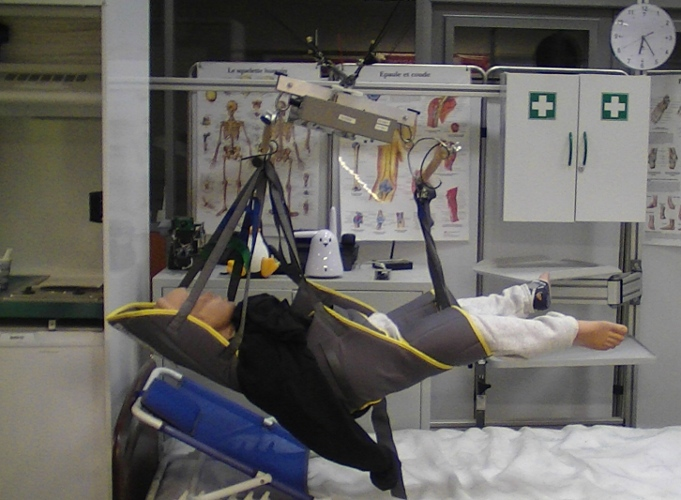
\includegraphics[width=.48\linewidth]{./chapter0/figures/case03.jpg}} \hfill
    \caption{\footnotesize{Différents types de fragilités motrices dans des 
situation de la vie quotidienne}}
\label{intro:fig8}
\end{figure}

Un dispositif répondant à ces impératifs doit présenter les caractéristiques 
suivantes :
\begin{itemize}
 \item pouvoir supporter des charges correspondant au poids d'une personne
 \item avoir un espace de travail équivalent à la taille d'une pièce de vie
 \item être léger et suffisamment discret et modulaire pour ne pas bouleverser 
l'environnement de l'utilisateur
 \item avoir une précision suffisante pour permettre un positionnement 
garantissant la sécurité, l'efficacité et le confort des opérations de 
transfert 
et d'attachement/détachement de l'utilisateur à la plate-forme.
\end{itemize}

Le choix d'utilisation d'un robot parallèle à câbles semble donc le plus 
compatible avec l'ensemble de ces exigences. {\tt Marionet-Assist} a ainsi été 
conçu et déployé dans un appartement-témoin 
(Fig.\ref{intro:fig10view0},\ref{intro:fig10view1}) situé dans les locaux 
de l'INRIA. Les câbles permettant le contrôle de la plate-forme sont fixés au 
plafond de l'appartement. Dans sa configuration actuelle, {\tt Marionet-Assist} 
est équipé de $4$ câbles, mais peut en contrôler jusqu'à $6$. Plusieurs 
stratégies sont envisageables au niveau des points de fixation sur la 
plate-forme :
\begin{itemize}
 \item les points d'attaches des câbles sont tous différents, il est alors 
possible avec $n$ câbles de contrôler $n$ degrés de liberté. Cette 
configuration.
sera notée $N-N$ (Fig.\ref{intro:fig9view0}).
 \item les câbles sont attachés en un même point à la plate-forme : il est 
posible à partir de $3$ câbles de contrôler les déplacement en translation de 
la plate-forme, mais plus son orientation ; l'utilisation de plus de $3$ câbles 
permet alors d'augmenter la taille de l'espace de travail. On parle dans ce cas 
de configuration N-1. 
(Fig.\ref{intro:fig9view1}).
 \item certains câbles seulement sont attachés en un même point sur la 
plate-forme. Dans le cas par exemple d'une disposition pour laquelle $3$ câbles 
sont atttachés en un même point $B_0$ et un quatrième câble relié à la 
plate-forme en un point $B_1$, cette configuration sera notée 4-3-1 
(Fig.\ref{intro:fig9view2}).
\end{itemize}

\begin{figure}[htp]
  \centering
  \subfloat[Configuration 4-4 : chaque câble est relié à la plate-forme en un 
point distinct]{\label{intro:fig9view0}
  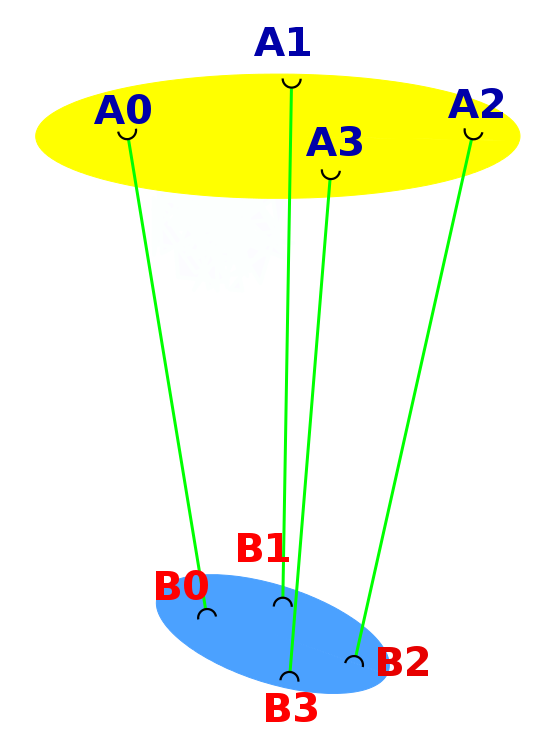
\includegraphics[width=.3\linewidth]{./chapter0/figures/cfg_44.png}} \hfill
  \subfloat[Configuration 4-1 : Les $4$ câbles sont reliés à la plate-forme un 
un seul point]{\label{intro:fig9view1}
  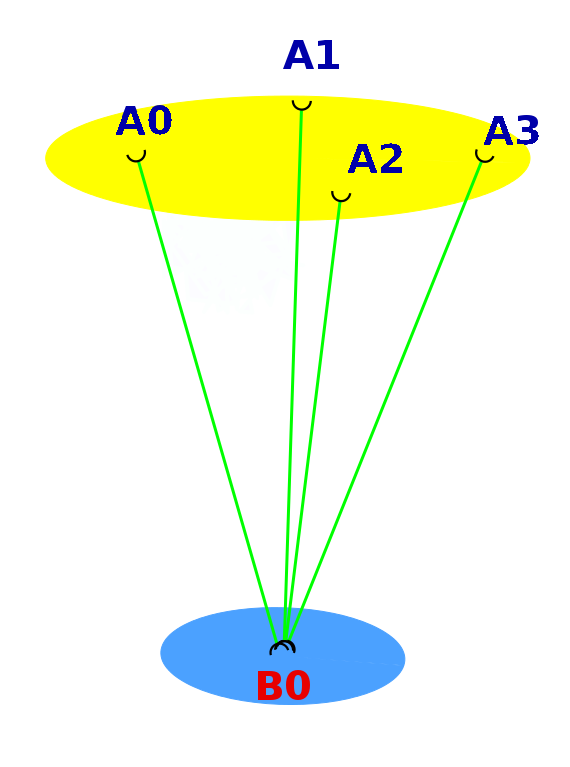
\includegraphics[width=.3\linewidth]{./chapter0/figures/cfg_41.png}}
  \subfloat[Configuration 4-3-1 : $3$ câbles sont reliés à la plate-forme en un 
même point, le quatrième est relié en un point distinct]{\label{intro:fig9view2}
  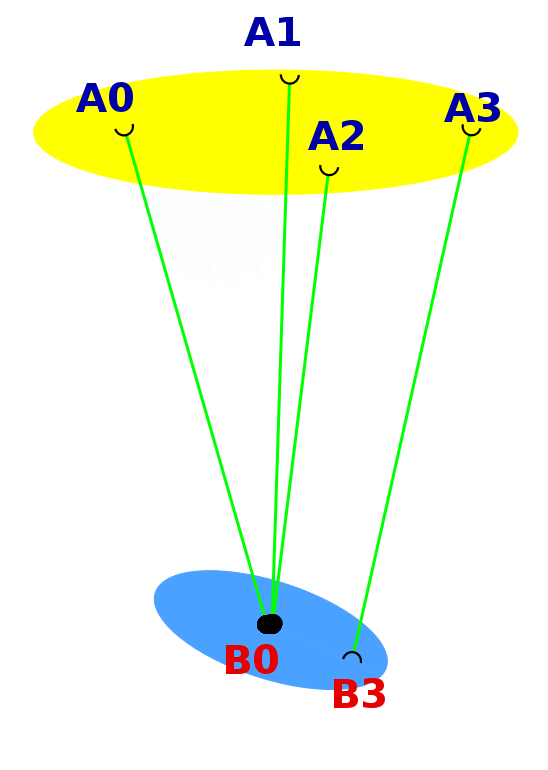
\includegraphics[width=.3\linewidth]{./chapter0/figures/cfg_431.png}} \hfill
    \caption{\footnotesize{Exemples de configurations avec $4$ câbles}}
\label{intro:fig9}
\end{figure}

Pour l'ensemble des expériences menées dans le cadre de ce travail, nous avons 
utilisé la configuration $4-1$ (Fig.\ref{intro:fig10view2}) qui nous permet de 
contrôler les déplacements en translation, le quatrième c\^able ayant été 
ajouté pour augmenter la taille l'espace de travail de manière à pouvoir se 
déplacer dans la quasi-totalité de l'appartement-témoin. Pour un triplet de 
c\^ables en tension, il est facile de montrer que l'\'equilibre statique est 
satisfait si le point ${\bf B}$ \`a sa projection dans le plan des ${\bf 
A}_i,{\bf A}_j,{\bf A}_k$ \`a l'int\'erieur du triangle constitu\'e par ces 
trois points. La figure (Fig.\ref{intro:fig11}) montre alors l'espace de 
travail 
atteignable pour chaque triplet de câbles en tension : on note qu'en tout point 
dont la projection verticale ne se trouve pas sur l'une des deux diagonales 
définies par les points $(A_0-A_2)$ et $(A_1-A_3)$, il existe pour chaque pose 
deux configurations possibles avec trois câbles en tension. Si la projection se 
trouve sur une diagonale, i lexiste une configuration qui a deux c\^ables en 
tension, \`a l'exception de l'intersection des diagonales pour laquelle nous 
avons deux configurations avec seulement deux c\^ables avec des $\tau > 0$.

\begin{figure}[!ht]
\centering
\def\svgwidth{.90\linewidth}
\input{./chapter0/figures/MA_corobots.pdf_tex}
\caption{\footnotesize{La figure au centre représente le robot {\tt 
Marionet-Assist} ; en bas à gauche est représenté l'espace de travail 
atteignable lorsque les câbles attachés aux points $A_0$, $A_1$, $A_3$ sont en 
tension, en bas à droite l'espace de travail atteignable pour les câbles reliés 
aux points $A_0$, $A_1$, $A_2$. En haut à gauche, nous avons l'espace de 
travail 
correspondant aux câbles $A_0$, $A_2$, $A_3$ en tension, et en haut à droite 
l'espace de travail atteignable pour les câbles attachés aux points $A_1$, 
$A_2$, $A_3$.}}
\label{intro:fig11}
\end{figure}

Les câbles sont en Kevlar, ce qui nous permet de négliger leur élasticité et de 
pouvoir les modéliser comme des jambes rigides lorsque leur tension est 
strictement positive. Le contrôle des longueurs se fait à l'aide de tambours 
actionnées par des moteurs rotatifs (Fig.\ref{intro:fig10view3}). Toutefois, en 
l'absence de guide pour l'enroulement, il existe des incertitudes sur la 
longueur déroulée ; afin de pallier à cet inconvénient, des rep\`eres en 
aluminium ont été disposés sur les câbles à des longueurs connues, ce qui 
permet lors de leur détection au point ${\bf A}_i$ de réactualiser la valeur 
estimée de la longueur déroulée.

\begin{figure}[htp]
  \centering
  \subfloat[Vue globale de l'appartement-témoin]{\label{intro:fig10view0}
  
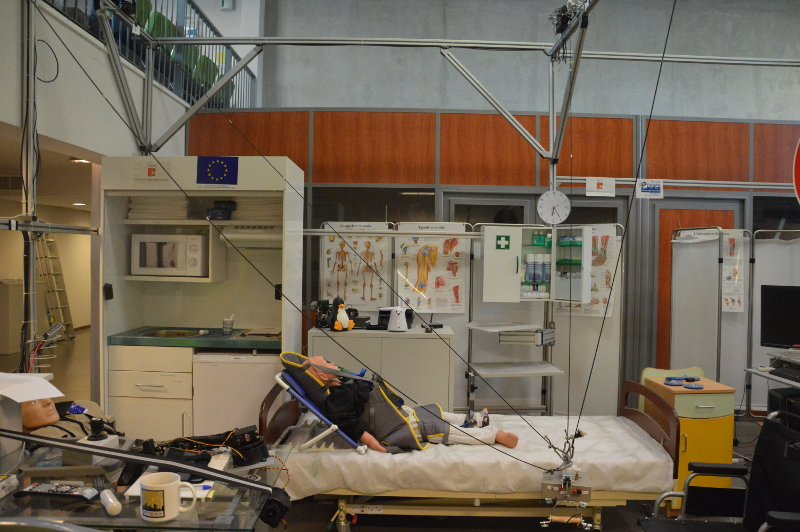
\includegraphics[width=.6\linewidth]{./chapter0/figures/view_appartment01.jpg}} 
\\
  \subfloat[Vue aérienne de l'appartement-témoin]{\label{intro:fig10view1}
  
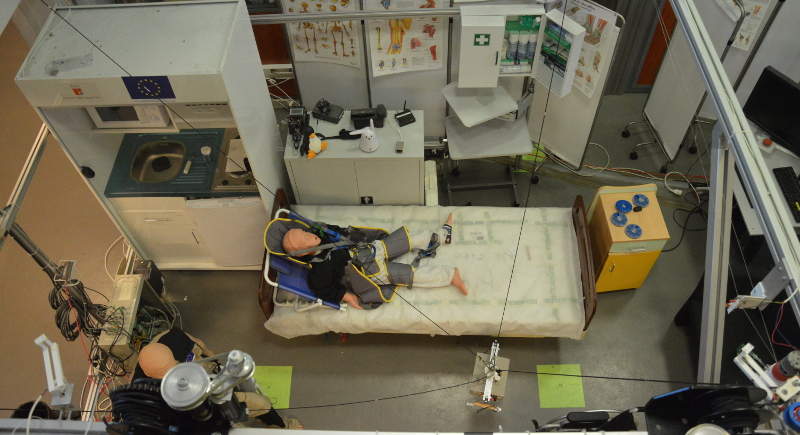
\includegraphics[width=.6\linewidth]{./chapter0/figures/view_appartment04.jpg}} 
\\
  \subfloat[Plateforme de {\tt Marionet-Assist}]{\label{intro:fig10view2}
  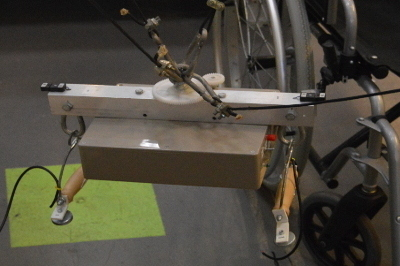
\includegraphics[width=.6\linewidth]{./chapter0/figures/view_plateform.jpg}} 
\\
  \subfloat[Système d'enroulement et actionneurs pour un 
câble]{\label{intro:fig10view3}
  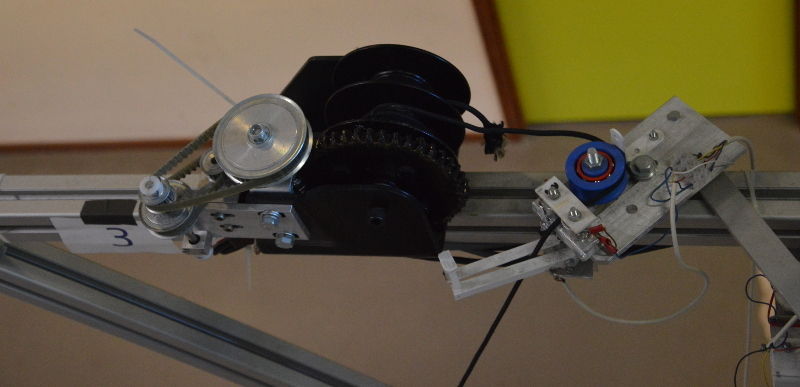
\includegraphics[width=.6\linewidth]{./chapter0/figures/view_winches02.jpg}}
    \caption{\footnotesize{{\tt Marionet-Assist}}}
\label{intro:fig10}
\end{figure}

Ces propriétés font de {\tt Marionet-Assist} un robot adapté au contexte pour 
lequel il a été conçu. Nous avons cependant souhaité améliorer ses 
fonctionnalités de manipulation en lui permettant de ne pas seulement déplacer 
une personne, mais également des objets de la vie quotidienne. Il peut s'agir 
par exemple de ramasser un objet tombé au sol, ou d'amener à l'utilisateur un 
objet (des lunettes par exemple) localisé à un endroit de la pièce éloigné de 
celui auquel il se trouve. Afin de localiser l'objet, puis de guider le robot 
dans son déplacement et dans la manipulation de l'objet cible, une caméra a été 
ajoutée sur la plate-forme, de manière à utiliser des techniques 
d'asservissement visuel. Ce sont ces dernières que nous allons à présent 
introduire, avant d'indiquer d'une part les problématiques posées par leur 
utilisation dans ce contexte particulier, et d'autre part les différentes 
possibilités d'améliorations que cela autorise concernant le contrôle des 
robots parallèles à câbles.

\section{Conclusion}

Apr\`es avoir mis en avant les inconv\'enients des architectures s\'eries pour 
certaines t\^aches, nous avons pr\'esent\'e dans un premier temps les 
architectures parall\`eles. Ces derni\`eres permettent en particulier de 
supporter de plus lourdes charges avec une pr\'ecision accrue, pour une taille 
du disposotif moindre. Les robots parall\`eles pr\'esentent cependant 
l'inconv\'enient d'\'evoluer dans un espace de travail restreint. Pour cette 
raison, l'utilisation de c\^ables a \'et\'e propos\'ee \`a la place de jambes 
rigides. Nous avons donc pr\'esent\'e les principales caract\'eristiques des 
robots parall\`eles \`a c\^ables, et identifi\'e les probl\'ematiques 
qu'entra\^inait le choix d'une telle architecture, au rang desquelles la 
complexit\'e accrue des mod\`eles g\'eom\'etriques et cin\'ematiques, ainsi que 
la difficult\'e \`a g\'erer la nature des tensions (nulles ou strictement 
positives) pour chaque c\^able. Enfin, nous avons introduit les 
sp\'ecificit\'es d'une clase particuli\`ere de manipulateurs \`a c\^ables : les 
robots N-1, dont fait parti le prototype que nous avons utilis\'e dans 
le cadre de ce travail, le robot {\tt Marionet-Assist}. Dans le chapitre 
suivant, nous introduirons les principales notions d'asservissement 
visuel, avant de nous pencher sur les specificit\'es d'une utilisation dans le 
contexte de robots parall\`eles \`a c\^ables. Nous pourrons d\`es lors 
clairement identifier les pistes d'am\'elioration de manipulation que 
association de ces deux technologies permet.

\vfill